%
% IT.
% Information Technology
%
% Aleph Objects Operations Manual
%
% Copyright (C) 2014, 2015 Aleph Objects, Inc.
%
% This document is licensed under the Creative Commons Attribution 4.0
% International Public License (CC BY-SA 4.0) by Aleph Objects, Inc.
%

\section{Network}
See figure \ref{fig:ao_net_overview} for an overview of Aleph Objects' network from May, 2015.
%See figure \ref{fig:ao_net_dot} for an Aleph Objects network diagram from 2015-05.
%See figure \ref{fig:ao_net_neato} for an Aleph Objects network diagram from May, 2015.
See figure \ref{fig:ao_net_sfdp} for a detailed Aleph Objects network diagram from 2015-05.
See figure \ref{fig:ao_net_dia} for an older Aleph Objects network diagram from February, 2014.

%\begin{sidewaysfigure}[p]
%\thisfloatpagestyle{empty}
%% The ao-network-overview.pdf built in calligraflow.
%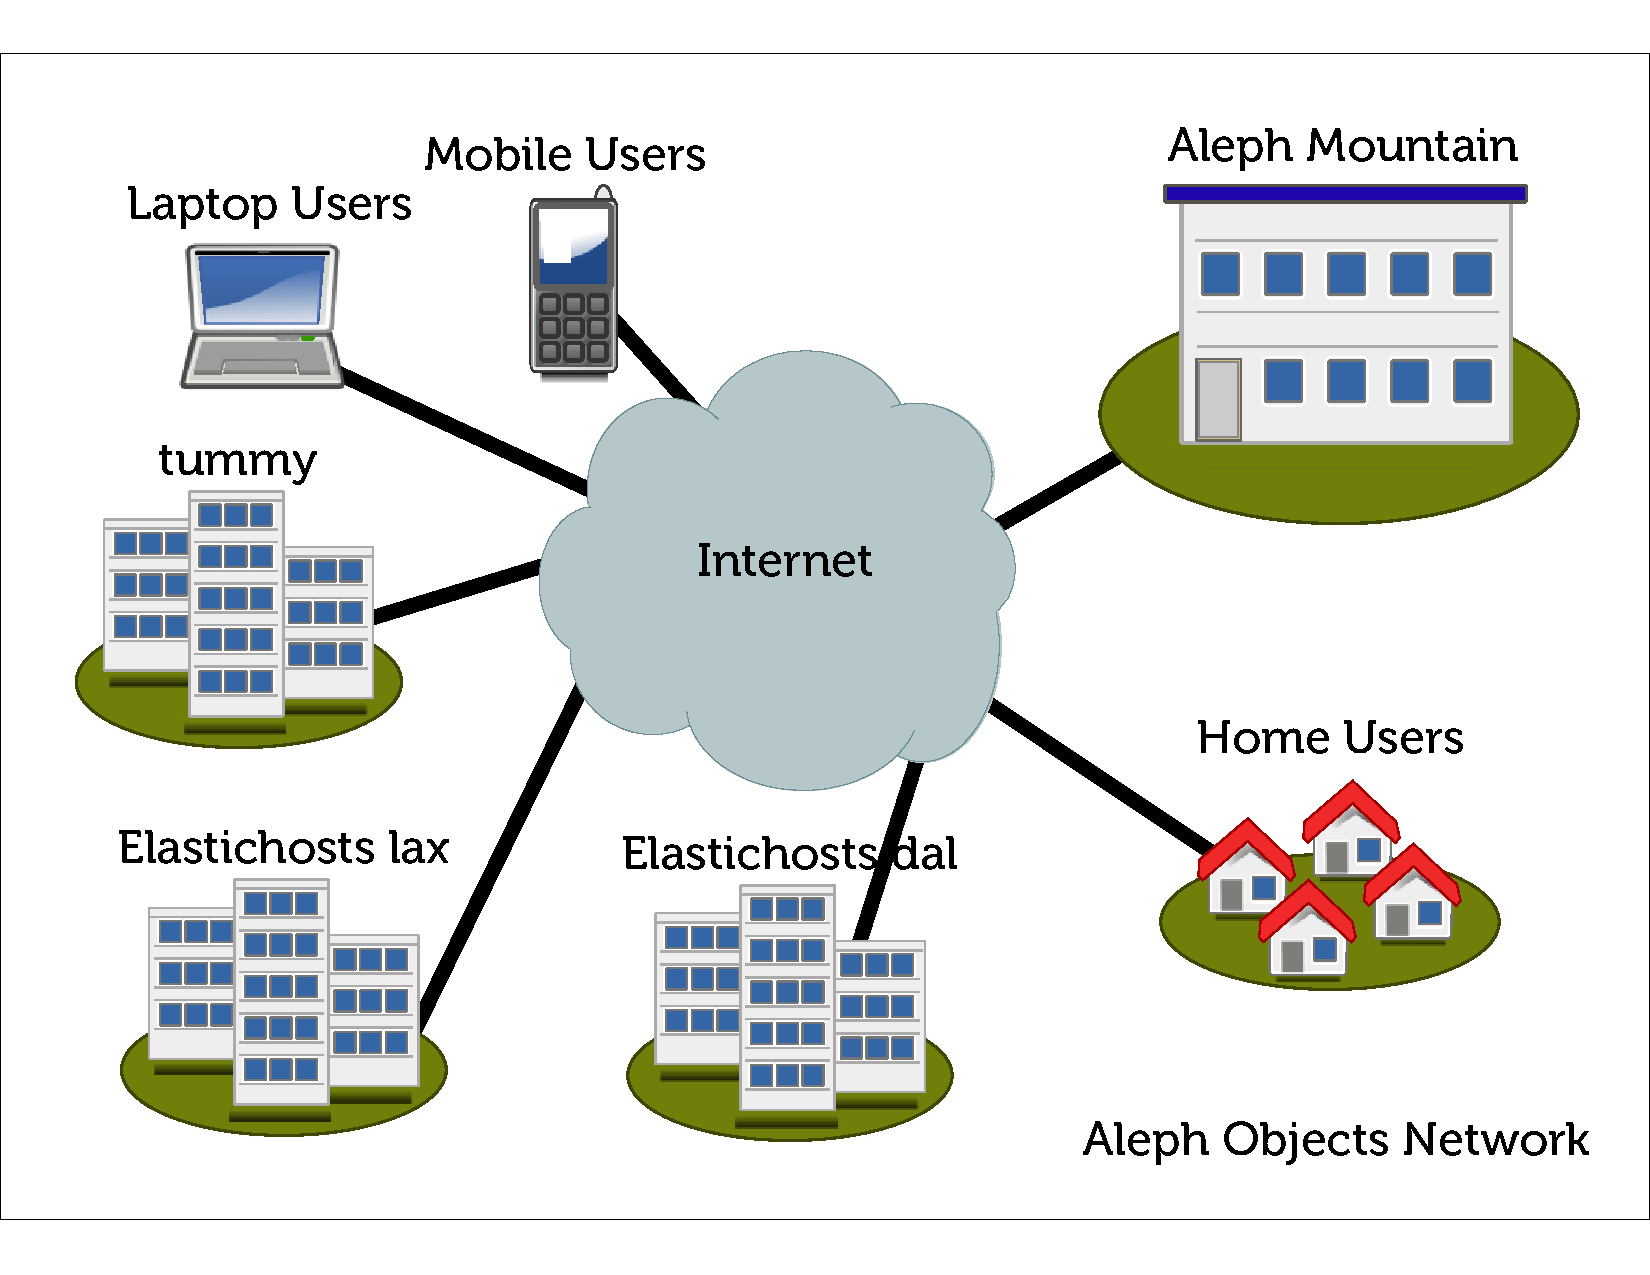
\includegraphics[keepaspectratio=true,height=1.10\textheight,width=1.00\textwidth,angle=0]{ao-network-overview.pdf}
% \caption{Aleph Objects Network Overview}
% \label{fig:ao_net_overview}
%\end{sidewaysfigure}

%\begin{sidewaysfigure}[p]
%\thisfloatpagestyle{empty}
%% The aonet-dot.png built with dot from aonet.dot source.
%
\includegraphics[keepaspectratio=true,height=1.10\textheight,width=1.00\textwidth,angle=0]{aonet-dot.png}
% \caption{Aleph Objects Network Overview, dot}
% \label{fig:ao_net_dot}
%\end{sidewaysfigure}

%\begin{sidewaysfigure}[p]
%\thisfloatpagestyle{empty}
%% The aonet-neato.png built with neato from aonet.dot source.
%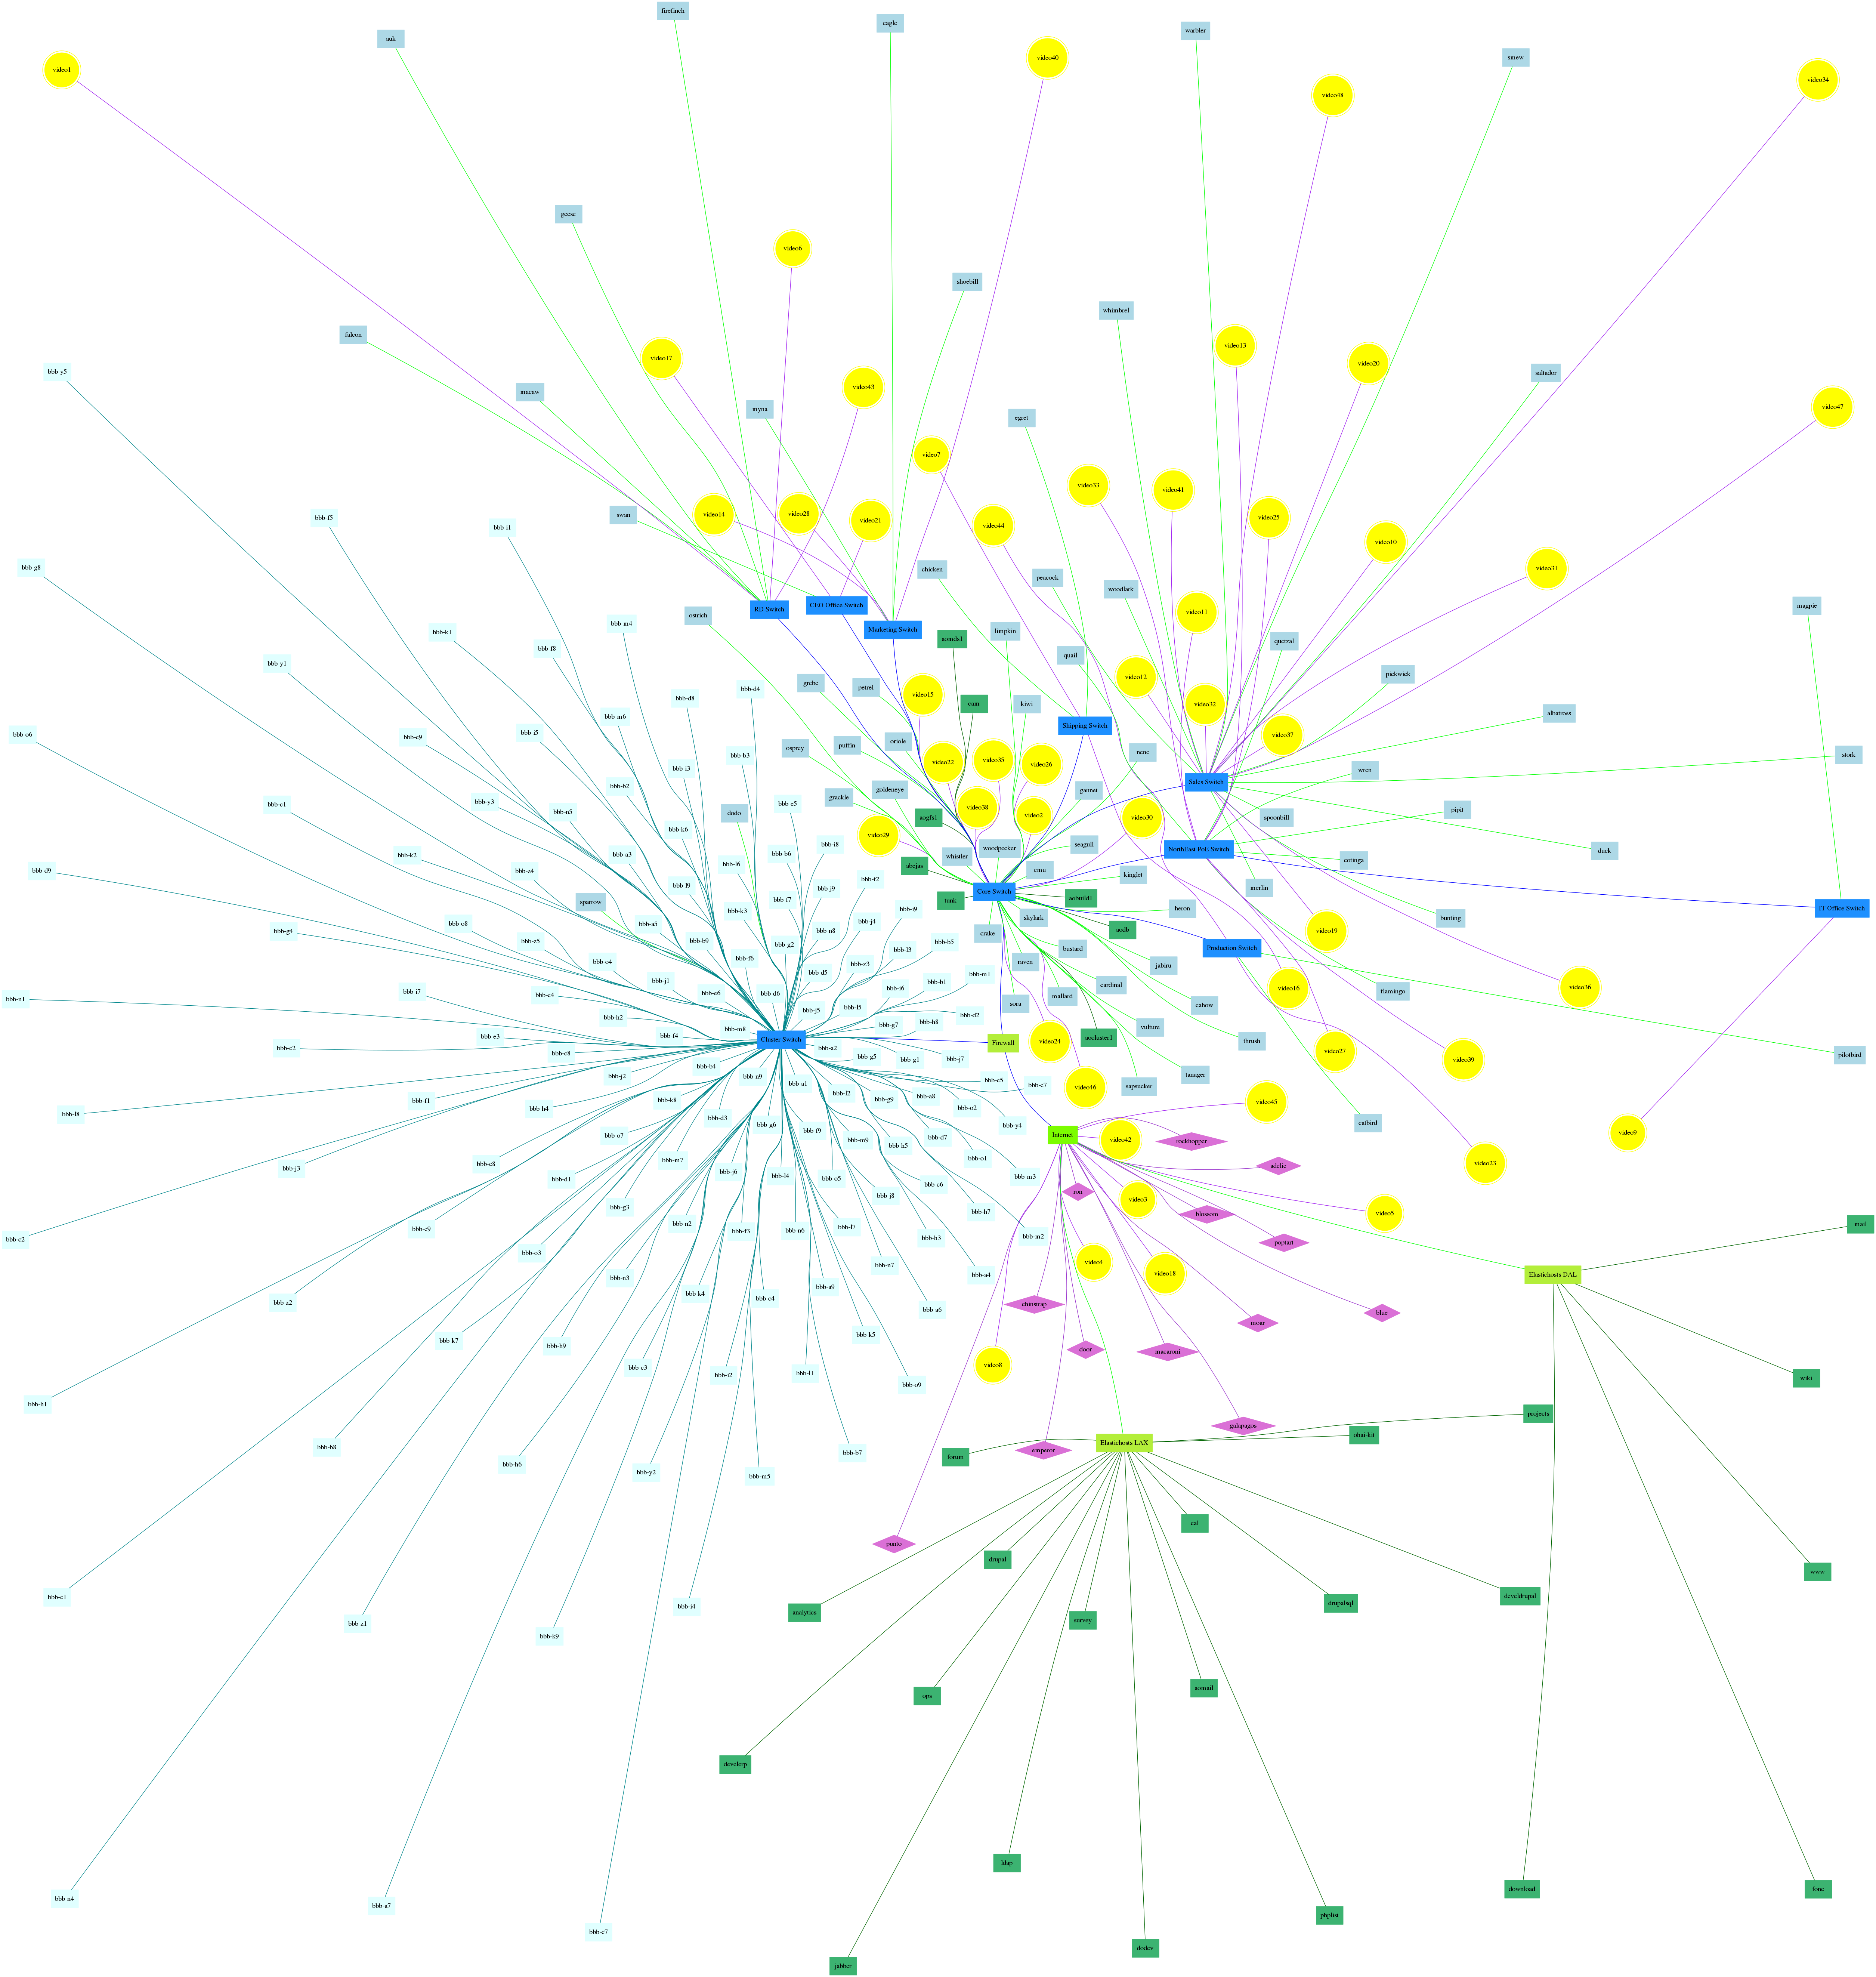
\includegraphics[keepaspectratio=true,height=1.10\textheight,width=1.00\textwidth,angle=0]{aonet-neato.png}
% \caption{Aleph Objects Network Overview, neato}
% \label{fig:ao_net_neato}
%\end{sidewaysfigure}

\begin{sidewaysfigure}[p]
\thisfloatpagestyle{empty}
% The aonet-sfdp.png built with sfdp from aonet.dot source.
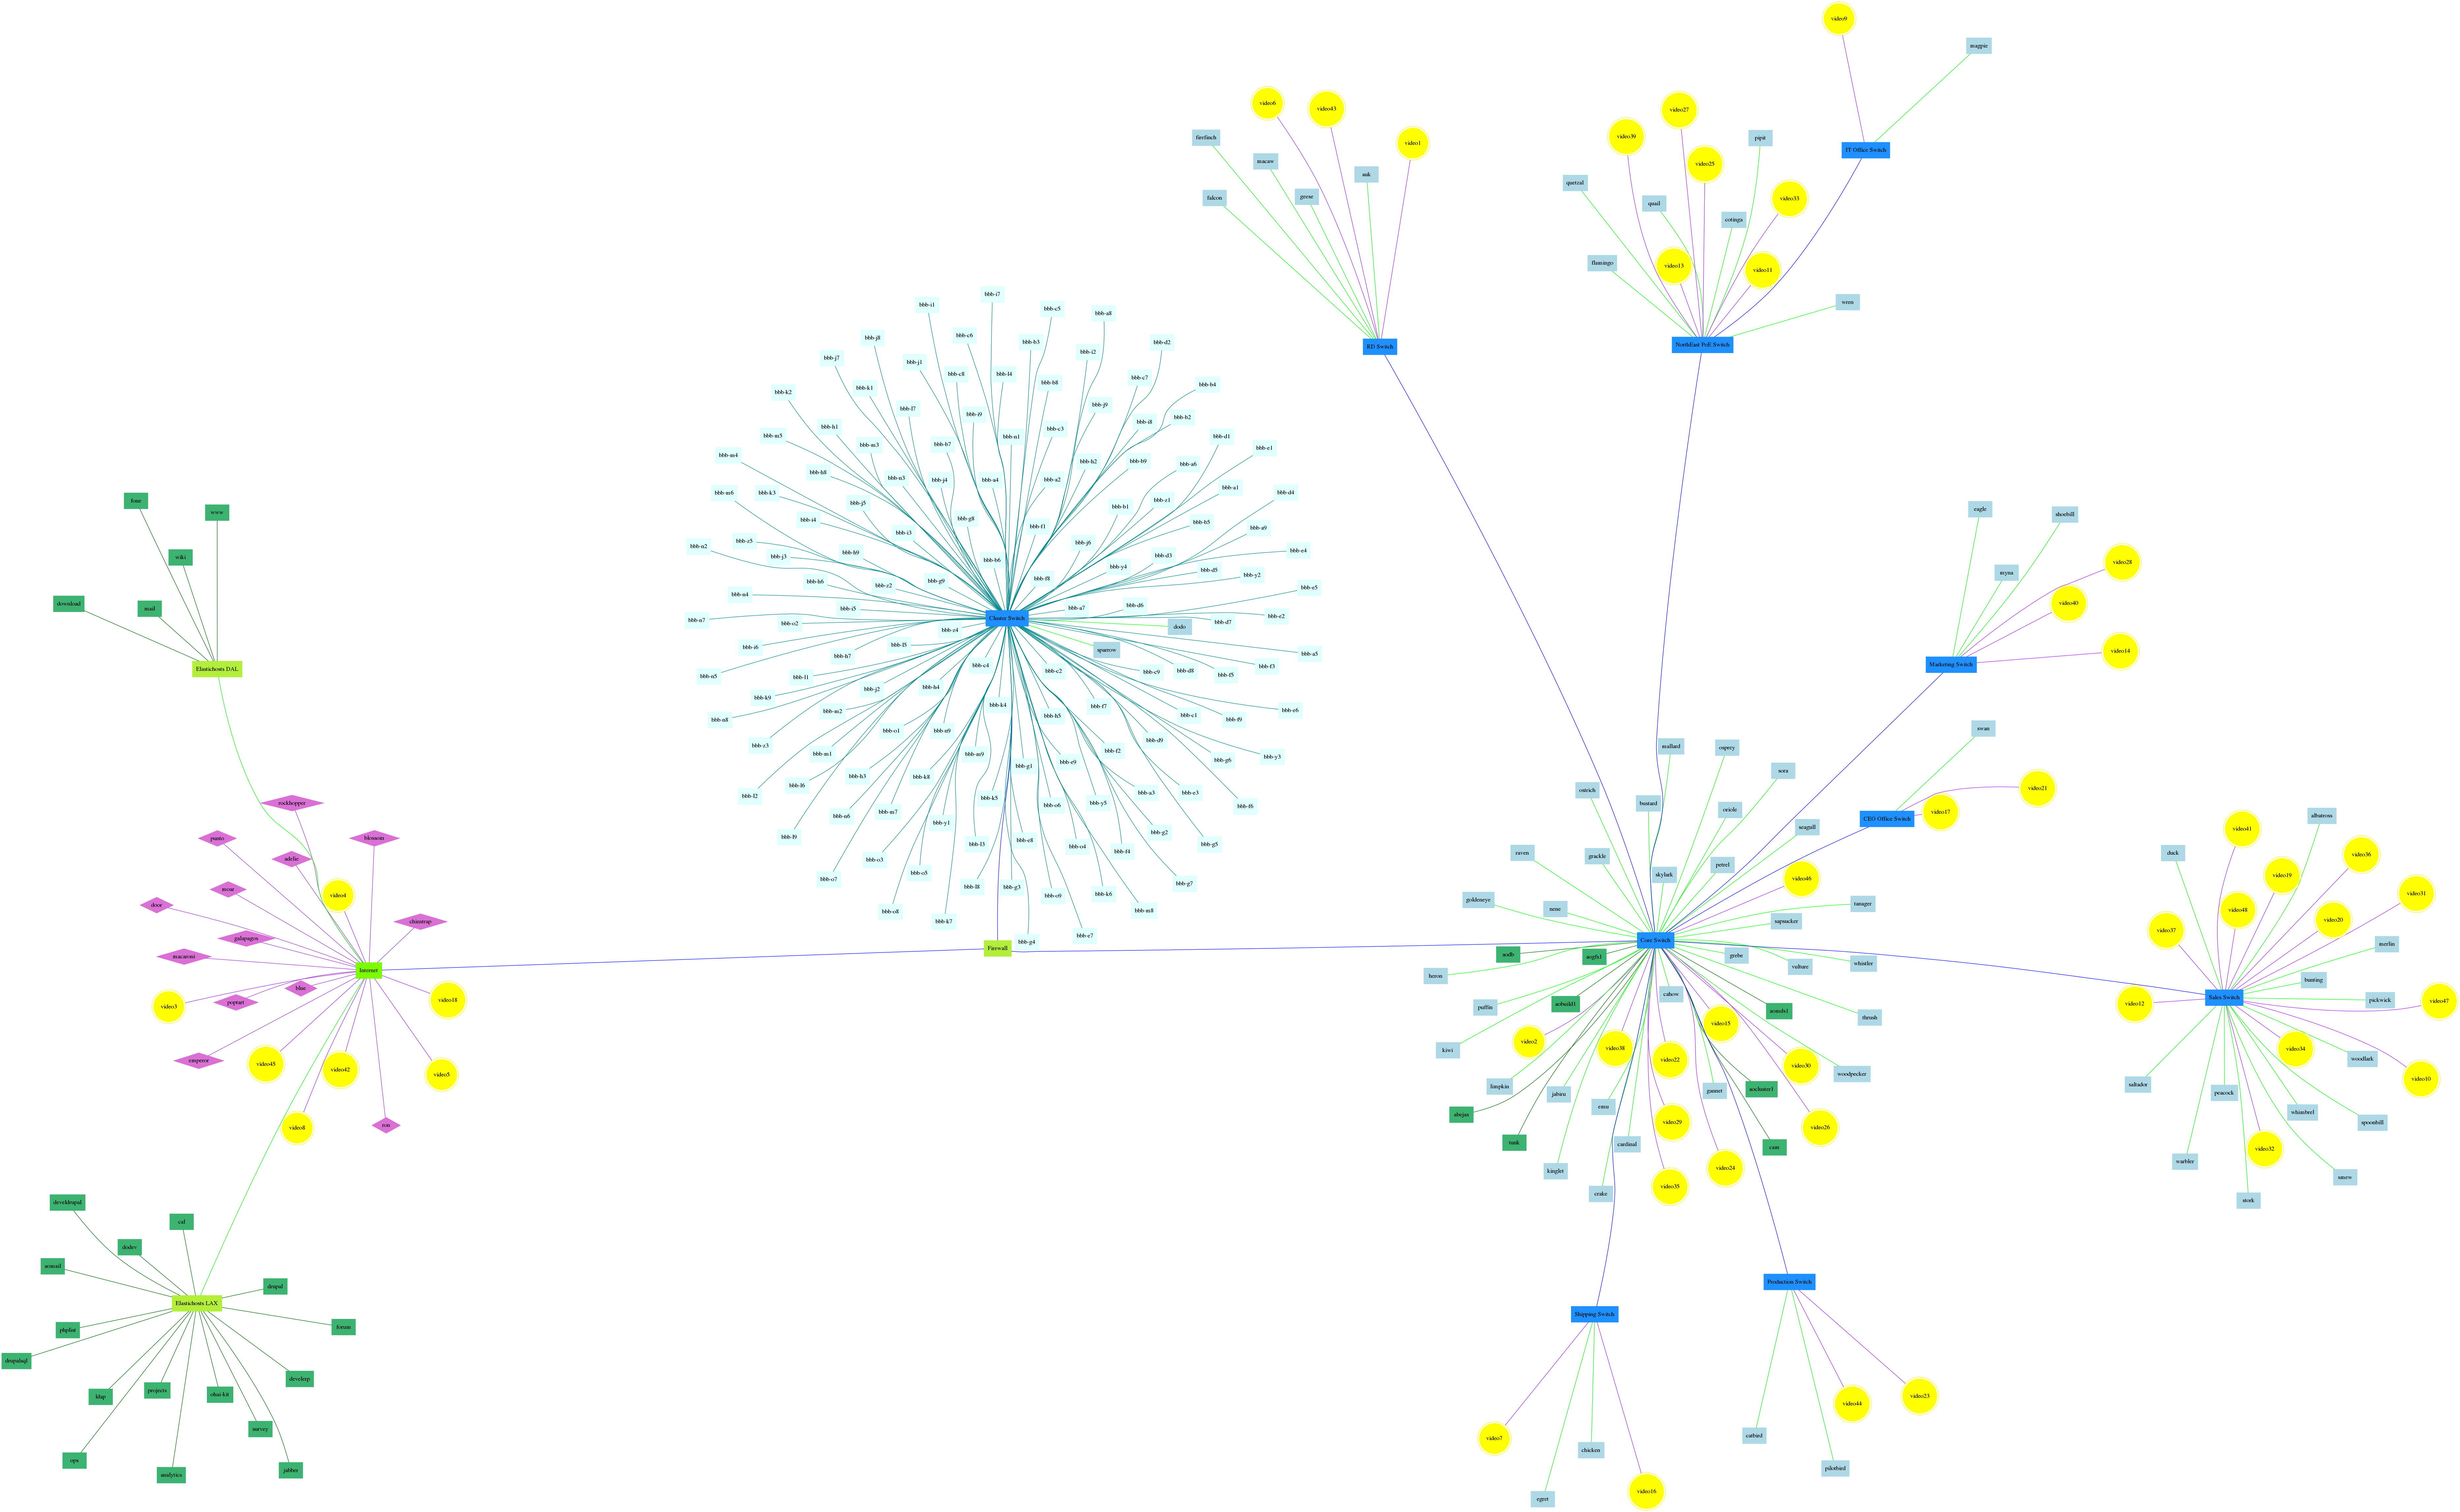
\includegraphics[keepaspectratio=true,height=1.10\textheight,width=1.00\textwidth,angle=0]{aonet-sfdp.png}
 \caption{Aleph Objects Network Detail, May 2015}
 \label{fig:ao_net_sfdp}
\end{sidewaysfigure}

\begin{sidewaysfigure}[p]
\thisfloatpagestyle{empty}
% The ao-network.pdf was built in Dia.
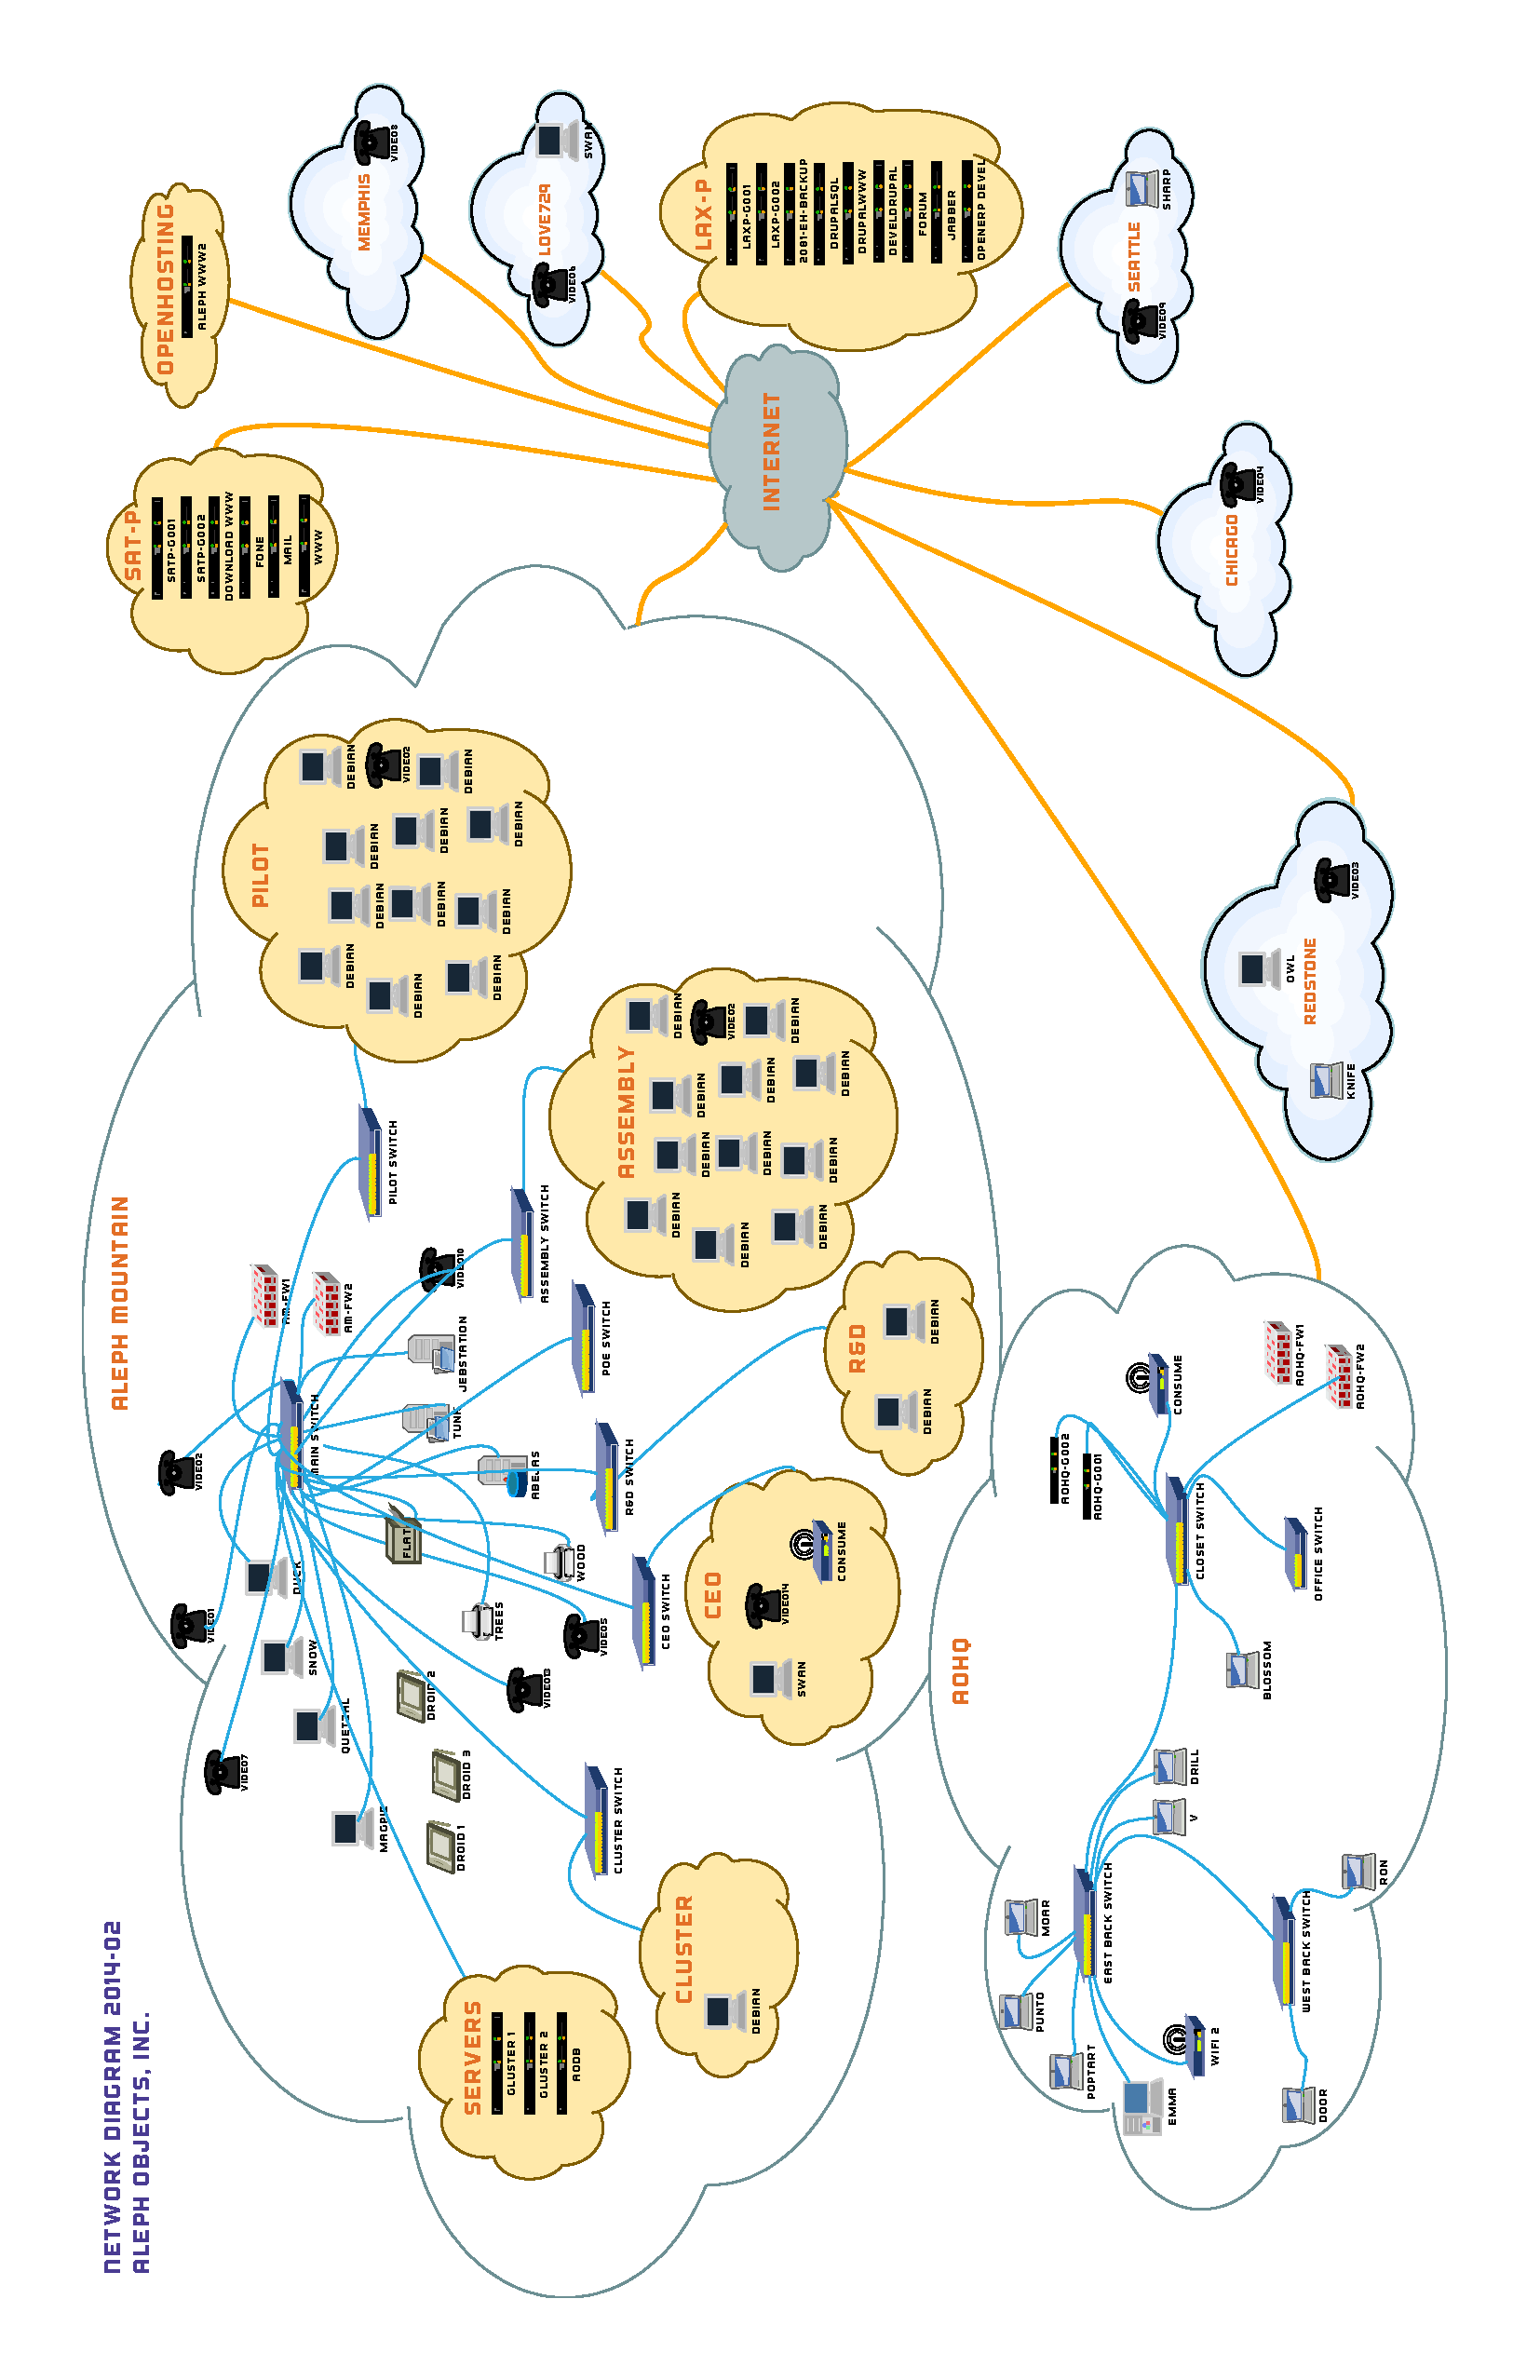
\includegraphics[keepaspectratio=true,height=1.10\textheight,width=1.00\textwidth,angle=-90]{ao-network.pdf}
 \caption{Aleph Objects Network Diagram, February 2014}
 \label{fig:ao_net_dia}
\end{sidewaysfigure}

